
\subsection{Linux - Etcher}

Das grafische Programm Etcher (\url{https://etcher.io}) kann zum �bertragen der Image-Datei verwendet werden. Es ist vor Allem f�r Anf�nger zu empfehlen, da beim Konsolenprogramm dd das Risiko besteht, dass Daten einer falschen Partition bzw. eines Laufwerks zerst�rt werden. Das Programm muss allerdings manuell installiert werden.     

\begin{console}
	wget https://github.com/resin-io/etcher/releases/download/v1.3.1/etcher-1.3.1-linux-x86_64.zip 
	unzip etcher-1.3.1-linux-x86_64.zip
	chmod +x etcher-1.3.1-x86_64.AppImage
	sudo mv etcher-1.3.1-x86_64.AppImage /usr/local/bin/etcher
	etcher &
\end{console}


Nach dem Starten wird danach gefragt ob eine Verkn�pfung zum Programm erstellt werden soll. Dies sollte man mit "`Yes"' beantworten. Danach kann man mit der Schaltfl�che "`Image"' die Image-Datei ausw�hlen. Ist nur ein m�gliches Ziel vorhanden, wird es bereits vorausgew�hlt, z.~B. die SD-Karte im Karten-Slot (/dev/memcblk0) oder im USB-Adapter (/dev/sdb). Sind mehrere m�gliche Ziele vorhanden, wird die "`Select Drive"' Schaltfl�che freigeschaltet. Dann kann ein Laufwerk manuell ausgew�hlt werden.

\begin{figure}[ht]
	\centering
	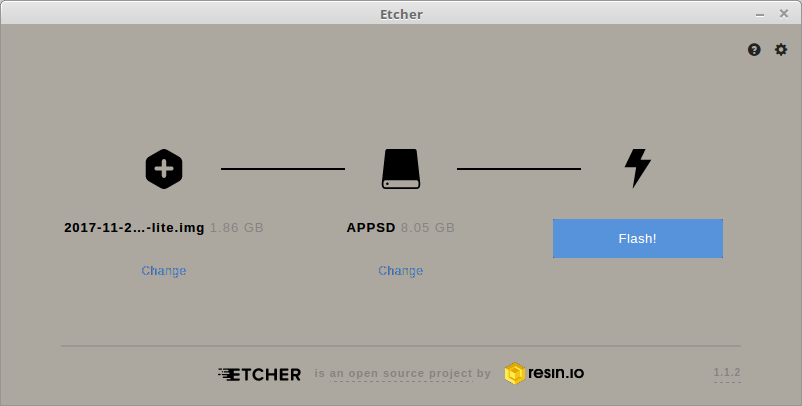
\includegraphics[scale=0.3]{images/Etcher_1.png}
	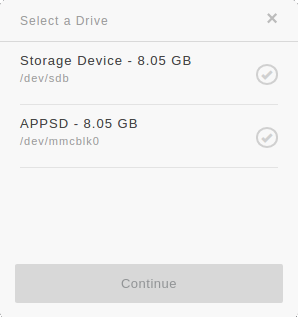
\includegraphics[scale=0.3]{images/Etcher_2.png}
	\label{Etcher}
\end{figure}


Wenn man noch etwas �ndern will, kann die entsprechende "`Change"' Schaltfl�che ausgew�hlt werden. Zum Schluss wird der Schreibvorgang mit der "`Flash!"' Schaltfl�che gestartet. M�glicherweise wird vom Programm allerdings noch das System-Passwort abgefragt.\\ 
Das Laufwerk bzw. die Partitionen werden nun aus dem System ausgeh�ngt und der Schreibvorgang gestartet. Der Fortschritt, die durchschnittliche �bertragungsrate und die Restlaufzeit werden w�hrend des Vorgangs angezeigt.\\ 


